% To je predloga za poročila o domačih nalogah pri predmetih, katerih
% nosilec je Tomaž Curk. Avtor predloge je Blaž Zupan.
%
% Seveda lahko tudi dodaš kakšen nov, zanimiv in uporaben element,
% ki ga v tej predlogi (še) ni. Več o LaTeX-u izveš na
% spletu, na primer na http://tobi.oetiker.ch/lshort/lshort.pdf.
%
% To predlogo lahko spremeniš v PDF dokument s pomočjo programa
% pdflatex, ki je del standardne instalacije LaTeX programov.

\documentclass[a4paper,11pt]{article}
\usepackage{a4wide}
\usepackage{fullpage}
\usepackage[utf8x]{inputenc}
\usepackage[slovene]{babel}
\selectlanguage{slovene}
\usepackage[toc,page]{appendix}
\usepackage[pdftex]{graphicx} % za slike
\usepackage[justification=centering]{caption}
\usepackage{setspace}
\usepackage{multicol}
\usepackage{color}
\definecolor{light-gray}{gray}{0.95}
\usepackage{listings} % za vključevanje kode
\usepackage{minted} % za barvanje kode
\usepackage{hyperref}
\renewcommand{\baselinestretch}{1.2} % za boljšo berljivost večji razmak
\renewcommand{\appendixpagename}{Priloge}


\newminted{ts}{
  % remove first 2 characters (padding spaces)
  gobble = 2,
  % set left line (code block padding hack)
  frame = leftline,
  % 0 width for frame ruler (gives padding but is invisible)
  framerule = 0pt,
  % distance between frame and content
  framesep = 8pt,
  % set background
  bgcolor = light-gray
}
% usage:
% \begin{tscode}
%   // Some great code.
% \end{tscode}

\title{\huge{Končno poročilo} \\ \Large{\em{Mreže v socialnem omrežju Vine}}}
\author{Marko Grešak (63130058)}
\date{\today}

\begin{document}

\maketitle

\section{Uvod}

V svoji projektni nalogi sem analiziral podatke socialnega omrežja \href{https://vine.co}{\underline{Vine}}. Pri tem je bilo eno bolj zanimivh področij problem, kako kar se da dobro prikazati sodelovanje uporabnikov. Poskušal sem tudi odkriti, kakšne skupnosti se tvorijo čez čas, vendar mi to zaradi pomanjkana podatkov ni uspelo. Pred začetkom idelave naloge sem po raziskavi ugotovil, da še nihče ni delal podobne raziskave oziroma je ni objavil javno.

\subsection{Kaj je Vine?}

Ko govorim o projektu se v večini primerov najprej pojavi vprašanje: \textit{“Kaj je Vine?”}. Vine je Twitterjeva spletna storitev, ki uporabnikom omogoča nalaganje do 7 sekundnih videov, s časom pa so ga uporabniki začeli uporabljati kot čisto neodvisno socialno omrežje. Omrežje je postalo popularno zaradi uporabnikov, ki ustvarjajo smešno vsebino.

\subsection{Podatki in Tehnologije}

\begin{itemize}
  \item Omejil sem se na uporabnike z vsaj 50.000 sledilci, teh sem našel 588,
  \item Za razvojno okolje sem si izbral \href{https://nodejs.org/}{\underline{Node.js}} in \href{http://www.typescriptlang.org/}{\underline{TypeScript}},
  \item Večino grafov sem narial iz Node.js s pomočjo storitve \href{https://plot.ly/}{\underline{Plotly}}, z izjemo grafa sodelovanja med uporabniki, ki je narisan s pomočjo \href{http://d3js.org/}{\underline{D3.js}}.
\end{itemize}

\subsection{Programska koda}
Programska koda je javno dostopna na GitHubu, na naslovu\\
\href{https://github.com/markogresak/vine-data-mining}{\underline{https://github.com/markogresak/vine-data-mining}}

\subsection{Pojmi}
\begin{itemize}
  \item API - \href{http://en.wikipedia.org/wiki/Application_programming_interface}{\underline{Application programming interface}},
  \item \href{http://sl.wikipedia.org/wiki/Predpone_SI}{\underline{k, M, B}} - 1.000 (tisoč), 1.000.000 (milijon), 1.000.000.000 (milijarda), v tem zaporedju.
\end{itemize}

\pagebreak
\section{Podatki}

\subsection{Izvor podatkov}

Med iskanem podatkov nisem našel nobene povezave, z že vnaprej pripravljenimi podatki. To pomeni, da vse svoje podatke črpam zgolj iz \href{https://api.vineapp.com}{\underline{Vine API}}. Ker API nima nikakršne uradne dokumentacije, sem si moral pomagati redkimi, predvsem pa zastarelimi, viri na spletu ter svojim raziskovenjam, iz tega pa sem izpeljal dokumentacijo \href{https://github.com/markogresak/vine-data-mining/blob/master/API-reference.md}{\underline{Vine API Reference}}. Že ob času pisanja tega poročila so nekatere informacije zastarele, ampak se jih nisem spravil popravljati, saj sem bil prezaposljen s popravljanjem same kode.
\par
Na tej točki sta se že pojavila prva dva problema: pomanjkanje dokumentacije ter večkratno spreminjanje API-ja, zaradi česar je vsa najdena dokumentcija hitro zastarela. Samo v času izdelave tega projekta se je po mojem opažanju odgovor API-ja spremenil vsaj trikrat. Sicer spremembe niso bile drastične, ampak so bile dovolj, da sem moral svoj program popravljati, da je lahko nadaljeval, pojavili pa so se tudi nekonsistentni podatki za iste odgovore APIja, zato sem se po drugi spremembi odločil, da ne shranjujem direktnih odgovorov, ampak svoje, prilagojene vrednosti.
\par
Naslednji problem se je pojavil pri ID vrednostih, saj so vse večje od limita vrednosti za številko v JavaScriptu oziroma TypeScript, jezik v katerem sem napisal mojo nalogo. Razlaga za to je, da je največja cela številčna vrednost v JavaScriptu \(2^{53}\), kar pa je manj od ID vrednosti, katera je bila npr. \textit{934940633704046592}, zato se je zgodil preliv (ang. overflow), na koncu pa je bila vrednost iz primera enaka \textit{934940633704046600}. To seveda pomeni, da uporabnika po tej vrednosti ne morem najti, saj je shranjena vrednost različna od pravega idja entitete, API pa seveda za podan ID odgovori s statusom napake.
\par
Problem sem rešil tako, da sem začel pri 5 po mojem mnenju najbolj sledenih uporabnikih, pri katerih je verjetnost sodelovanja večja, saj imajo veliko število objav. Pri zaključevanju sem ugotovil, da sem spustil samo enega uporabnika, ki je imel več sledilcev, pa še ta je pred kratkim skril svoje objave, torej si z njegovimi podatki ne bi veliko pomagal.
\par
Za vsakega od teh uporabnikov sem pripravil zahtevo na profil ter hkrati na časovnico, kjer se nahajajo vsi posnetki. Na le-tej se pojavi omejitev, saj lahko v zahtevi dobimo največ 100 posnetkov, za več pa moramo zahtevati naslednje strani. Problem sm rešil preprosto, saj ob vsaki zahtevi kot odgovor dobim število vseh objav, potem pa preostale izračunam po formuli \(\left \lfloor{\frac{n}{100}}\right \rfloor\) , kjer je \textit{n} število vseh objav, navzdol pa zaokrožim, ker prvo skupino objav že imam.

\subsection{Programsko zbiranje podatkov}

Ker je uporabnikov in Vine posnetnov ogromno, z vsakim novim pa se število potrebnih zahtev povečuje zelo hitro, sem si naprej postavil omejitev, da uporabnike z manj od 10k sledilcev preskočim. To se je kasneje izkazalo za prenizko mejo, zato sem jo povišal na 50k, saj se drugače zbiranje podatkov ne bi končalo v nekem doglednem času, da bi lahko zaključil predstavitev.
\par
Odločil sem se izdelati mrežo računalnikov, oziroma instanc strežnikov, ki bodo zbirale podatke ter jih oddajale na centralni, zmogljivejši strežnik. To se je izkazalo za zelo slabo idejo, saj sem za razvoj tega sistema skupno porabil okoli 50 ur, ko pa sem sistem prvič pognal, je bilo toliko zahtev, da se je sistem sesul v manj kot pol ure. Poskusil sem z najzmogljivešim strežnikom na DigitalOcean, ki so mi ga dovolili najeti, ampak tudi tam zgodba ni bila dosti drugačna. Nazadnje sem se odločil vzpostaviti strežnik kar na svojem osebnem računalniku, saj je bil glavni problem RAM in diskovni prostor, tega pa imam več, kot strežnik, ki sem ga najel. Poleg tega sem v vmesnem času še dodal nekaj optimizacij, zato se je rešitev za nekaj ur že kazala obetavne rezultate. Ampak je število zahtev rastlo ``brez meja'', v okoli 48 urah neprestanega delovanja se je izvajanje še vedno zdelo, da sem daleč od konca, zato sem se odločil delovanje ustaviti in pregledati podatke. Zbral sem skoraj dva GB podatkov s skupno več kot 5M vnosi. Čeprav sem se trudil in implementiral več mehanizmov za preprečeavnje shranjevanja duplikatov, je bilo še vseeno okoli 10\% podatkov podvojenih, prav tako pa je bila večina podatkov o posnetkih.
\par
Tu sem se odločil izbrati samo podatke o uporabnikih ter dodal že prej omenjeno mejo za 50k sledilcev, prav tako pa sem iz množice izključil uporabnike, ki so imeli zasebne profile, kar pomeni, da ni možnosti pridobivanja vseh zanimivh informacij o njihovem profilu. Napisal sem tudi manjšo skripto, ki opravlja delo celotnega prej opisanega sistema, saj je le-ta težko obvladljiv, poleg tega pa tudi nisem potreboval visoke zmogljivosti, saj je zbiranje za \textit{588} preostalih uporabnikov trajalo okoli pol ure, na koncu pa sem zbral \textit{145.970} videov.

\section{Vizualizacije podatkov}

Zbrane podatke sem združil skupaj po uporabnikih ter jih uporabil za upodobo vizualizacij. Za test sem opravil še probno vizualizacijo za prejšnje, večje, podatke, s katero sem ugotovil, da se je uporaba manjšega seta bolj popularnih uporabnikov izkazala za dobro odločitev. Pri zadnjih se pojavijo bolj vidni vzorci razvoja popularnosti uporabnika, kot tudi razvoja same platforme. Prav tako pa se vidi kdaj je postala vsebina uporabnika viralna, pojav, ki se pri manj popularnih uporabnikih pojavi zelo redko ali celo nikoli.

\subsection{Uporbniki skozi čas}

Ena meni najbolj zanimivih vizualizacij, za katero sem zaradi nekonsistentnosti pri datumih tudi porabil kar nekaj časa, je prikaz grafa ogledov objavljenih objav skozi čas za deset najbolj popularnih uporabnikov, od začetka februarja 2013, kar je nekaj dni po uradnem odprtju omrežja Vine, do konca maja 2015. Na tem grafu se lepo vidi kako je z razvojem portala rastlo tudi število ogledov teh uporabnikov, prav tako pa so zelo nazorno vidni skoki ogledov, kar ponazarja, da so bili nekateri posnetki ogledani nadpovprečno velikokrat, torej so postali viralni.
\par
Tukaj bi še dodal, da so imena uporabnikov nekoliko popačena, saj platforma plot.ly ne podpira posebnih znakov v besedilu, zato sem se odločil izbrisati vse znake, ki niso črke.
\par
Za boljši pregled nad grafom proporočam klik na povezavo za interaktiven ogled. Če platforma zahteva prijavo, lahko pojavno okno zaprete in si graf ogledate tudi kot anonimni uporabnik.

\pagebreak

\begin{figure}[htbp]
  \begin{center}
    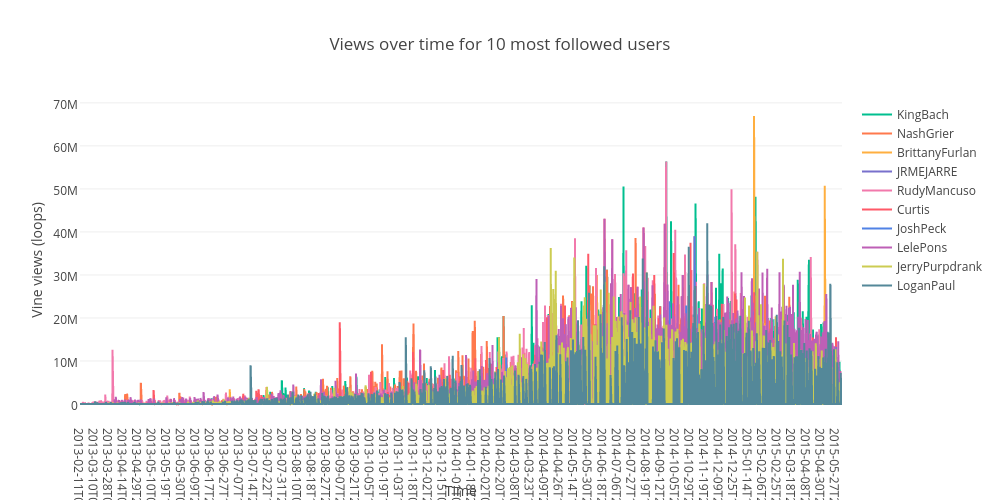
\includegraphics[width=\textwidth,height=\textheight,keepaspectratio]{figures/views-over-time.png}
    \caption{10 najbolj popularnih uporabnikov in njihovi ogledi skozi čas\\
    Interaktivni pregled: \href{https://plot.ly/~markogresak/61}{\underline{https://plot.ly/{\sim}markogresak/61}}}
  \end{center}
\end{figure}

\subsection{Sodelovanje med uporabniki}

Izrisal sem tudi graf sodelovanja med uporabniki, za katerega sem pričakoval, da bo prikazal kako so uporabniki povezani med seboj in kakšne mreže se tvorijo, ampak sem z vizualizacijo spoznal, da je sodelovanj med popularnimi uporabniki toliko, da se ne oblikujejo skupine, ampak so vsi uporabniki prepleteni med seboj, graf na sliki 2 pa zgleda kot klobčič volne.
\par
Šele na vizualizaciji uporabnikov z več od 5M sledilcev, katerih sem zajel samo 20, se vidijo povezave, ki jih lahko vidimo ter analiziramo. Debelina črte ponazarja večje število sodelovanj med povazanima uporabnikoma. Iz slike lahko vidimo, da uporabniki veliko sodelujejo med seboj, s tem pa si tudi pomagajo pri pridobivanju še več sledilcev.

\begin{figure}[htbp]
  \begin{center}
    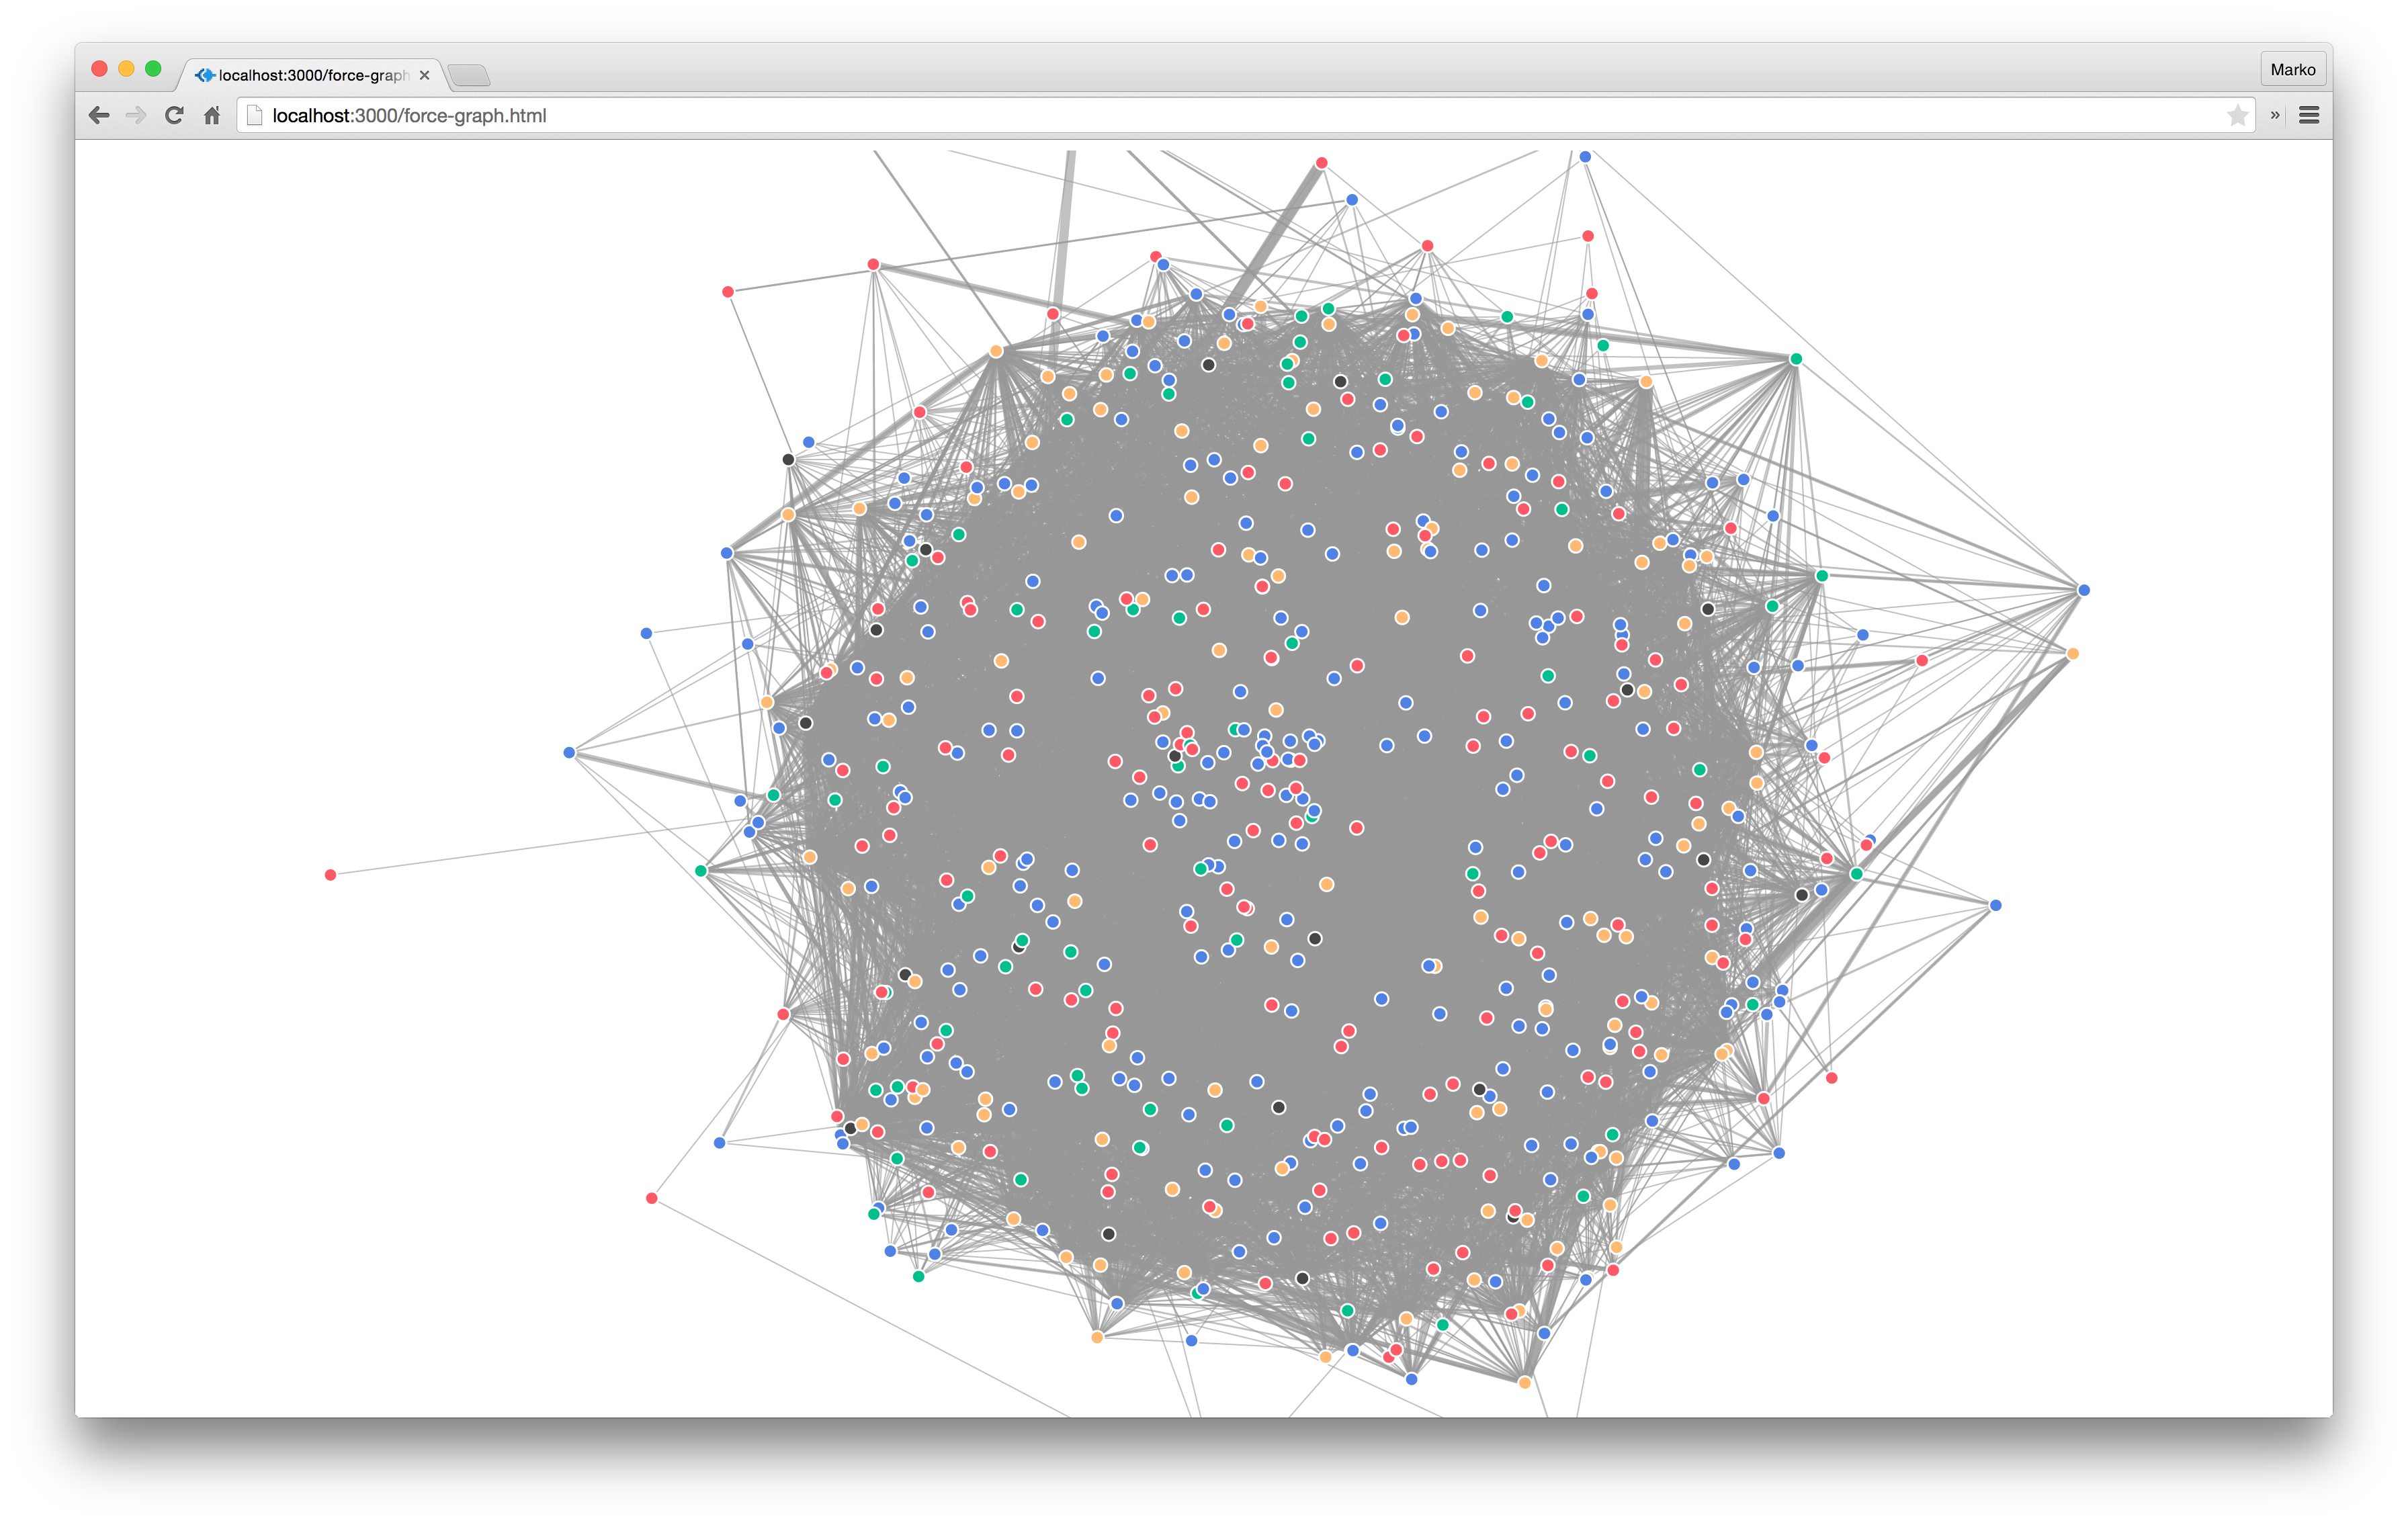
\includegraphics[width=\textwidth,height=\textheight,keepaspectratio]{figures/collaborations-all.png}
    \caption{Sodelovanje med vsemi uporabniki\\
    Interaktivni pregled (opcija all 588 users): \href{https://gresak.io/pr/graf-sodelovanja}{\underline{https://gresak.io/pr/graf-sodelovanja}}}
    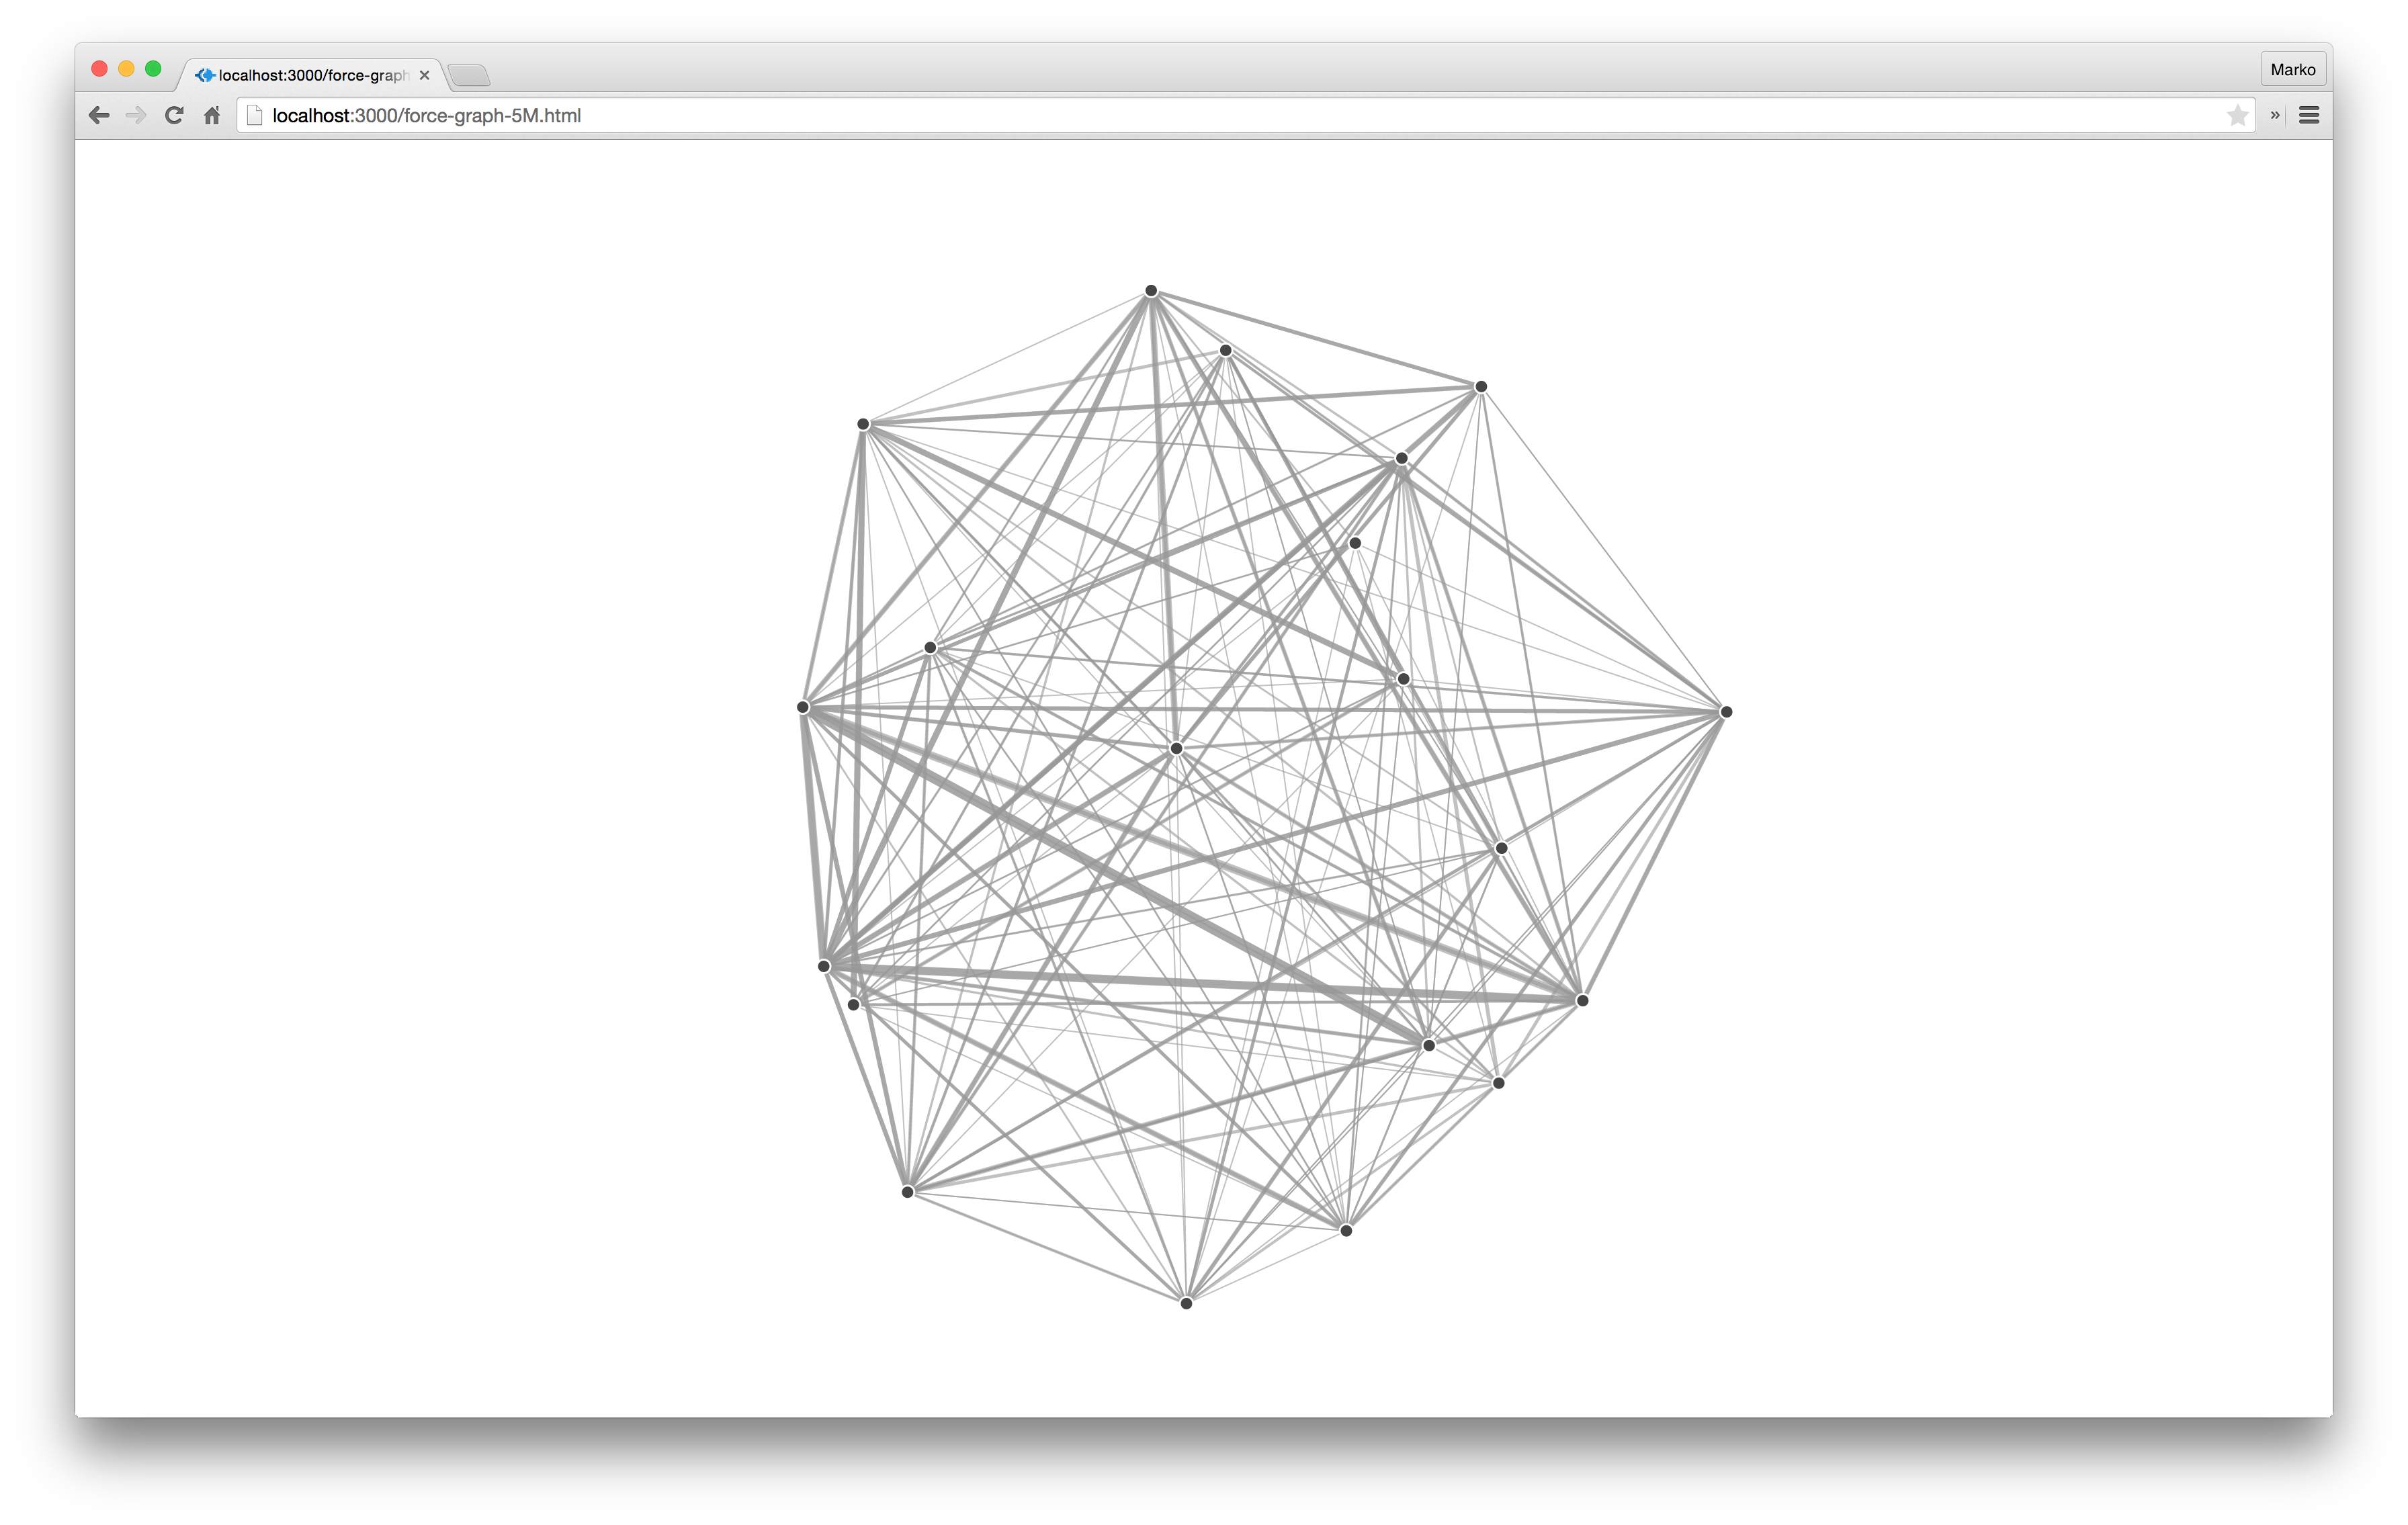
\includegraphics[width=\textwidth,height=\textheight,keepaspectratio]{figures/collaborations-over-5M.png}
    \caption{Sodelovanje med uporabniki z več kot 5M sledilcev\\
    Interaktivni pregled (opcija users over 5M): \href{https://gresak.io/pr/graf-sodelovanja}{\underline{https://gresak.io/pr/graf-sodelovanja}}\\
    \textit{(Če se graf ne prikaže, z miško premaknite prikazano točko.)}}
  \end{center}
\end{figure}

\pagebreak

\subsection{Ostale vizualizacije}

Poleg tega sem izrisal še nekaj vizualizacij, ki predstavljajo različne razporeditve glede na število sledilcev uporabnika, si lahko ogledate v prilogi.

\subsection{Vizualizacije, katerih nisem uspel izdelati}

Pri vmesni predstavitvi sem predlagal tudi vizualizacijo pogostosti objav na zemljevidu Združenih Držav Amerike, vendar sem po bolj podrobni analizi podatkov ugotovil, da to ne bo mogoče, saj je edina informacija o lokaciji uporabnika ta, ki jo uporabnik vnese v svoj opis kot besedilo, torej je to lahko karkoli, na primer naslov za drugo socialno omrežje, dodaten opis profila in podobno. Sicer sem še vseeno poskusil poiskati lokacije z \href{https://developers.google.com/maps/documentation/business/geolocation/}\underline{Google Geolocation API}, vendar je stopnja pravilnosti podatkov tako nizga, da se mi ni zdela vizualizacija got zanimiva.

\section{Izjava o izdelavi domače naloge}
Domačo nalogo in pripadajoče programe sem izdelal sam.

\pagebreak
\appendix
\appendixpage
\pagenumbering{gobble}

\section{Ostale vizualizacije}

\begin{figure}[htbp]
  \begin{center}
    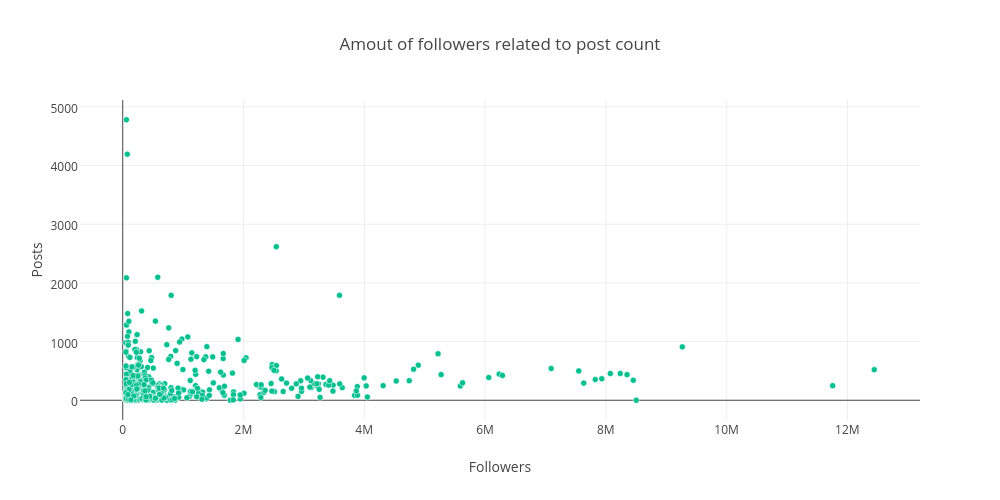
\includegraphics[width=\textwidth,height=\textheight,keepaspectratio]{figures/follower-posts.png}
    \caption{Razmerje med številom sledilcev ter številom objav\\
    Lahko nekaj osamelcev čisto pri vrhu na levi, to so računalniki, ki nalagajo ``spam'' ali ukradeno vsebino za všečke. \\
    Interaktivni pregled: \href{https://plot.ly/~markogresak/18}{\underline{https://plot.ly/{\sim}markogresak/18}}}
  \end{center}
\end{figure}

\begin{figure}[htbp]
  \begin{center}
    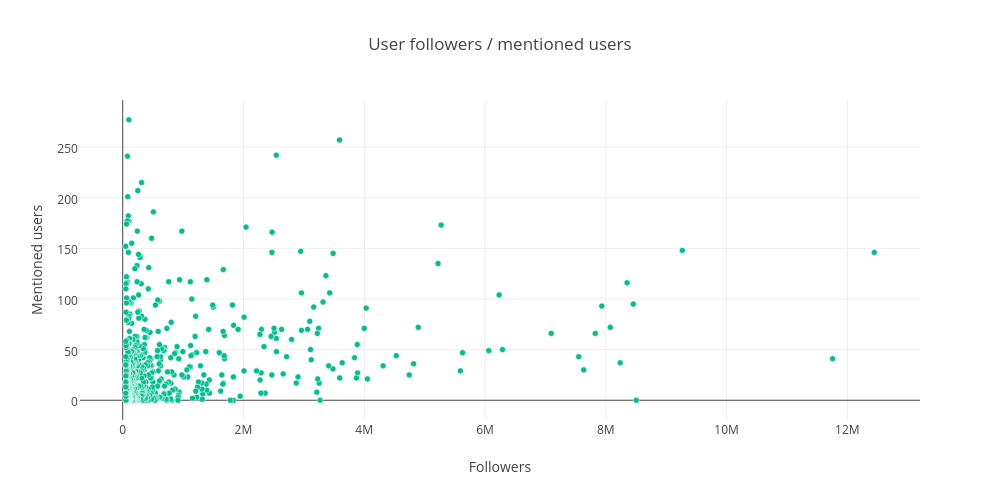
\includegraphics[width=\textwidth,height=\textheight,keepaspectratio]{figures/follower-cooperations.png}
    \caption{Razmerje med številom sledilcev ter sodelovanji z ostalimi\\
    Hitro lahko opazimo, da v povprečju s številom sledilcev narašča tudi število sodelovanj. \\
    Interaktivni pregled: \href{https://plot.ly/~markogresak/62}{\underline{https://plot.ly/{\sim}markogresak/62}}}
  \end{center}
\end{figure}

\begin{figure}[htbp]
  \begin{center}
    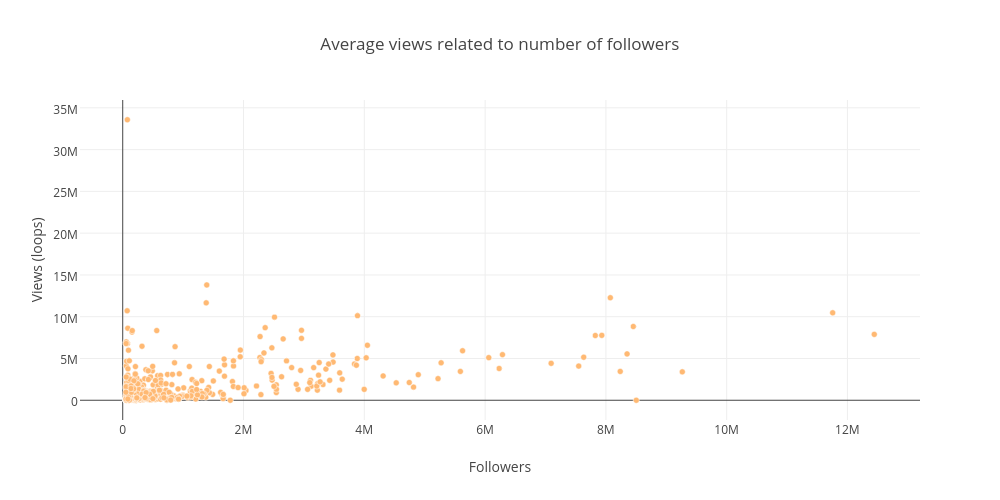
\includegraphics[width=\textwidth,height=\textheight,keepaspectratio]{figures/follower-avg-views.png}
    \caption{Razmerje med številom sledilcev ter povprečjem ogledov\\
    Zanimivi outlierji, po ročnem pregledu sem ugotovil, da so to slavne osebnosti, ki pa niso redno aktivne na Vine-u. \\
    Interaktivni pregled: \href{https://plot.ly/~markogresak/117}{\underline{https://plot.ly/{\sim}markogresak/117}}}
  \end{center}
\end{figure}

\begin{figure}[htbp]
  \begin{center}
    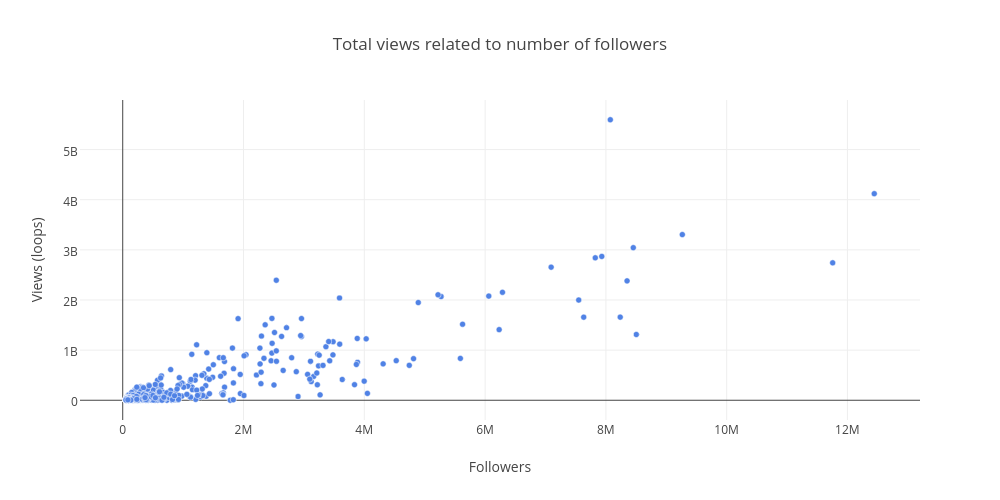
\includegraphics[width=\textwidth,height=\textheight,keepaspectratio]{figures/follower-total-views.png}
    \caption{Razmerje med številom sledilcev ter številom vseh ogledov\\
    Število vseh ogledov narašča skoraj linearno, izstopa pa avtorica, ki pogosto objavi vsebino, katero je potrebno pogledati večkrat za popolno razumevanje, predvsem zaradi hitrega dogajanja. \\
    Interaktivni pregled: \href{https://plot.ly/~markogresak/118}{\underline{https://plot.ly/{\sim}markogresak/118}}}
  \end{center}
\end{figure}

\end{document}
